\documentclass{article}
\usepackage{ragged2e} %段落两端自动对齐的包
\usepackage{graphicx} %插入图片的包
\author{XiaoLei WuZheng}
\title{Explaining the Stern-Gerlach Experiment with Quantum Mechanics}

\begin{document} 
\maketitle 
\vspace{8pt} 
\renewcommand{\abstractname}{\huge \quad }
\begin{abstract} 
\centerline{\large\textbf{Abstract}}
\normalsize
{The Stern-Gerlach experiment has played an extremely essential role in the physical micro-world. In this article, we’ll attach high importance to explain Stern-Gerlach experiment by quantum mechanics. }
\noindent 
\end{abstract}


\section{Introduction}
 \begin{center}
 \normalsize
 {The Stern-Gerlach experiment, which started from Otto Stern in 1921 and then finished by Otto.Stern and Walter Gerlach in 1922. It has an inhomogeneous magnetic field made by a magnet with a pointed pole tip and then send a beam through the apparatus, the beam of particles will be split into a number of beams. Surprisingly, experimental observations is completely beyond the expectations of the experimental designers. How to understand and explain the S.G experiment phenomenon is beneficial for us to learn quantum mechanics. We’ll explain the result through a theoretical framework of QM.}
 \justifying
 \end{center}
 
\section{Stern-Gerlach experiment}
 \subsection{Single S.G experiment}
  \paragraph
  \normalsize
  {The earliest motivation of this experimentation was proving a conception from Bohr. At that time, the beam should be dispersed over a vertical distance in classical physics prediction, such as picture a. However, It has been observed that the beam magically splits into two parts, one corresponding to the spin up and one corresponding to the spin down as picture b shows. We must work out the effect of the magnetic field on the beam. Because the interaction energy of the magnetic field is just ---${{\mu}\cdot{B}}$, the z-component of the force experienced by the atom is given by a equation(1). The observed z component of spin has only two possible values, spin up and down, respectively called Sz+  and Sz-. The two possible values are multiples of the basic angular momentum unit.Therefore, the reason, why classical physic gets a wrong prediction, is  Spatial quantization. It means that S.G experiment revealed quantization of electron spin angular momentum. It has been known that the orbital angular momentum quantum number is an integer, while the Stern-Galach experiment shows that the spin angular momentum quantum number is a half integer.}
   \begin{equation}
     $$ \[F_z = \frac{\partial \left(\mu \cdot B\right)} {\partial z} = \mu_z  \cdot \frac{\partial B_z}{\partial z} \] $$
   \end{equation}    
     
  
%插入图片
 \graphicspath{E://sg1.png}%外层大括号可写多个路径
 \begin{figure}[!h]%!h是不让图片直接显示在页面顶部
 \centering%居中显示
 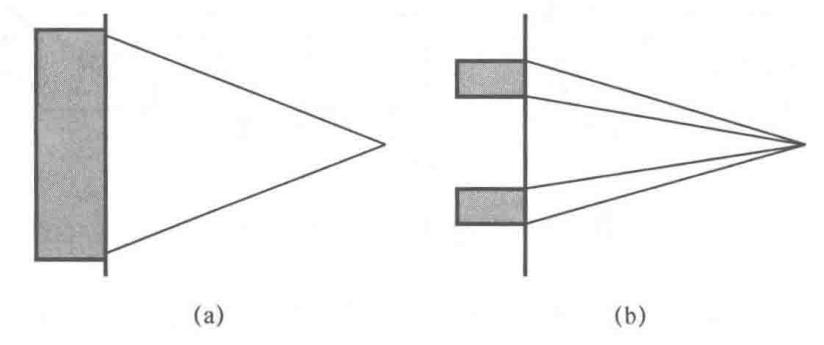
\includegraphics[width=0.6\textwidth ,height=1.5in]{E://sg1.png}%width和height设置长宽
 \end{figure}


 \subsection{Sequential Stern-Gerlach Experiments}
  \paragraph
  \normalsize
  {Now, let’s consider a sequential Stern-Gerlach experiment. As following figure shows, the beam goes through two or more SG apparatuses in sequence. [1]The first arrangement we consider is relatively straightforward. Like figure (a), we subject the beam coming out of the oven to the arrangement, where SGˆz stands for an apparatus with the inhomogeneous magnetic field in the z-direction. Then we block the Sz- component coming out of the first SGˆz apparatus and let the remaining Sz+ component be subjected to another SGˆz apparatus. This time there is only one beam component coming out of the second apparatus—just the Sz+ component. This is perhaps not so surprising; after all if the atom spins are up, they are remain so. The second arrangement is interesting shown in Figure 1.b. The Sz+ beam that enters the second apparatus (SGˆx) is split into two components, an Sx+ component and an Sx- component, with equal intensities. The third step is shown in Figure (c) which most dramatically illustrates the peculiarities of quantum-mechanical systems. This time we add to the arrangement of Figure (b) yet a third apparatus, of the SGˆz type. It is observed experimentally that two components emerge from the third apparatus, not one; the emerging beams are seen to have both an Sz+ component and an Sz- component. Obviously, we can’t determine both Sz and Sx simultaneously. More precisely, we can say that the selection of the Sx+ beam by the second appratus(SGˆx) compeletely destroys any precious information about Sz.}


 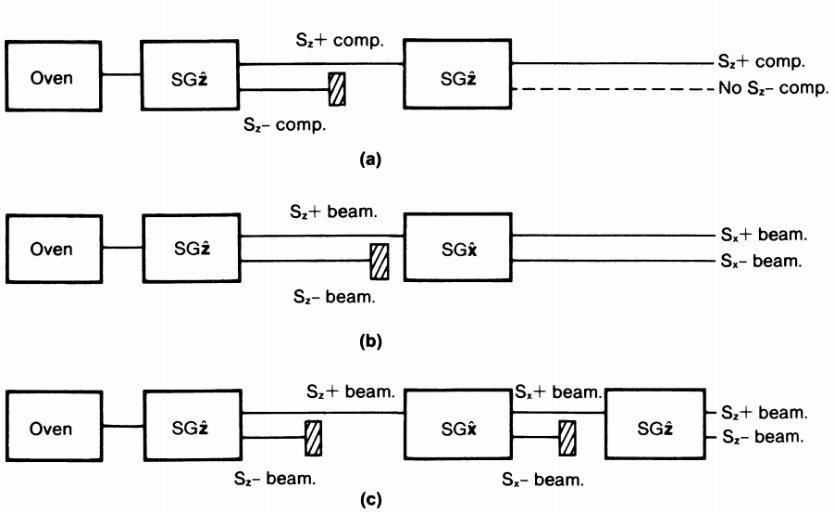
\includegraphics[width=1.1\textwidth]{E://sg2.png} %注意路径
  
\section{Conclusion}
 \normalsize
 \paragraph
 \normalsize{Stern-Gerlach experiment phenomenon could be explained by a basic principle in quantum mechanics. The priciple is blowing: Any atomic system can be separated by a filtering process into a certain set of what we will call base states, and the future behavior of the atoms in any single given base state depends only on the nature of the base state---it is independent of any previous history.}
 
\bibliographystyle{plain}   %参考文献命令行
%\cite{university1994dimension}        %参考文献的生成,快速构建*1+BibTex*1+快速构建*1(保留cite语句)
                                      %不知道为什么,最后生成pdf时,conclusion下方多了[1],注释掉cite语句后,再一次快速构建就解决了。。。。。。
\bibliography{sg} %sg.bib文件

 
\newpage
\end{document}
